\section{Introduction}
\label{sec:introduction}

%\begin{figure}
%  \centering
%  \begin{subfigure}[b]{0.25\textwidth}
%    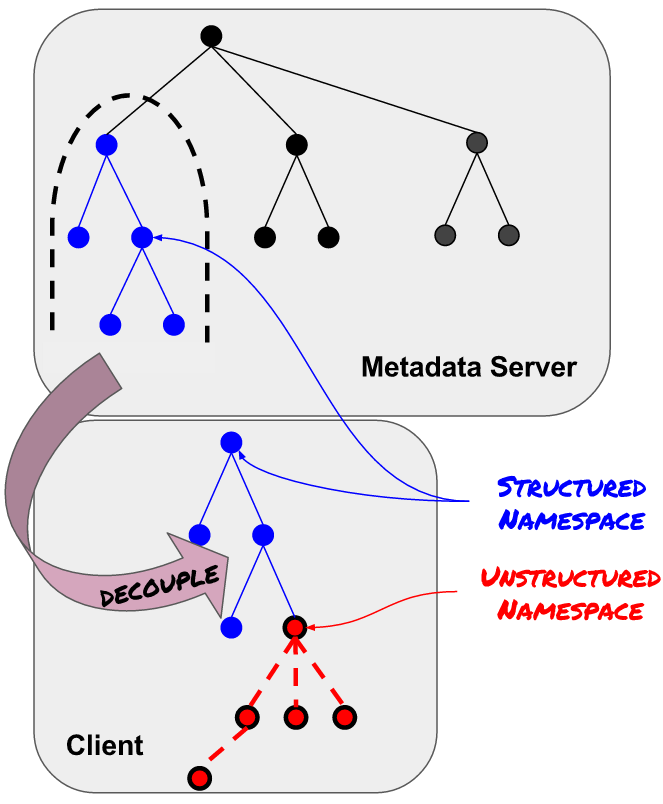
\includegraphics[width=\textwidth]{figures/intro.png}
%   \label{fig:intro}
%  \end{subfigure}
%  ~ 
%  \begin{subfigure}[b]{0.3\textwidth}
%    \begin{tabular}{ r | l }
%      Type         & Overhead       \\\hline\\
%      Structured   & 1 RPC          \\
%      Namespace    & O(1)           \\\\\hdashline\\
%      Unstructured & 1 RPC + Replay \\
%      Namespace    & O(1)           \\\\\hdashline\\
%      Traditional  & \(n\) RPCs     \\
%      Namespace    & O(\(n\))       \\
%    \end{tabular}
%    \\\\\\ % I am a hack
%   \label{table:intro}
%  \end{subfigure}
%  \caption{Clients decouple the file system subtrees and interact with their
%  private copiese locally for high performance. They can specify the structure of
%  the metadata they intend to create (structured namespace) or they can create
%  ad-hoc metadata (unstructured namespace), which is merged later.}
%\end{figure}
%    \caption{Traditional namespaces require at least 1 RPC per metadata
%    operation. Structured namespaces only need the initial RPC so clients/servers
%    understand (and can construct) the namespace.  Unstructured namespaces cannot
%    be parallelized and must replay metadata one by one onto the global namespace}

The file system metadata service is the scalability bottleneck for many of
today's workloads~\cite{roselli:atec2000-FS-workloads,
abad:techreport2012-fstrace, abad:ucc2012-mimesis,
alam:pdsw2011-metadata-scaling, weil:osdi2006-ceph}.  Common approaches for
attacking this ``metadata scaling wall" include: caching inodes on clients and
servers~\cite{depardon:tech13-survey, sinnamohideen:atc2010-ursa,
hildebrand:msst2005-pnfs, devulapalli:ipdps07-pvfs2, welch:fast2008-panasas},
caching parent inodes for path traversal~\cite{patil:fast2011-giga+,
ren:sc2014-indexfs, brandt:msst2003-lh, weil:sc2004-dyn-metadata,
ren:sc2014-indexfs}, and dynamic caching policies that exploit workload
locality~\cite{xing:sc2009-skyfs, zhu:pds2008-hba, li:msst2006-dynamic}.  These
caches reduce the number of remote procedure calls (RPCs) but the effectiveness
is dependent on the overhead of maintaining cache coherence and the
administrator's ability to select the best cache size for the given workloads.
We present an approach that, for certain workloads, reduces the number of RPCs
from O(\(n\)) to O(\(1\)), where \(n\) is the number of metadata accesses. Our
approach does not use a cache, so we do not encounter the same pain points of
maintaining a cache.

% What is our solution
We propose Tintenfisch, a file system that allows users to succinctly express
the structure and patterns of the metadata they intend to create.  Using this
semantic knowledge, Tintenfisch can optimize performance by reducing the number
of RPCs needed for (1) metadata writes because clients/servers can create
metadata independently and (2) metadata reads because clients can construct
metadata and pull data directly from the object store. Figure~\ref{fig:intro}
provides an architectural overview: clients first decouple the file system
subtree they want to operate on\footnote{This is not a contribution as it was
presented in~\cite{sevilla:ipdps18-cudele}.} then clients and metadata servers
lazily generate subtrees as needed using a ``namespace generator". The
namespace generator is stored in the root inode of the decoupled subtree and
can be used later to efficiently merge new metadata (that was not explicitly
state up front) into the global namespace. This workflow is essentially a
contract between clients and servers that relaxes durability and consistency
requirements.

The fundamental insight is that the client and server both understand the final
structure of the file system metadata so there is no need to communicate.  As a
consequence, less work is done on the metadata servers and clients help process
some of the metadata load.  The idea uses concepts from decoupled
namespaces~\cite{zheng:pdsw2014-batchfs, zheng:pdsw2015-deltafs} and patterned
IO~\cite{he:hpdc13-plfs-patterns} to build a scalable global namespace. The
actual implementation is similar to predicate push downs in databases, where
structure is described to lower storage layers using XML or
JSON~\cite{shel:pc17-pushdown}. Our contributions are as follows:

\begin{figure}[t]
  \centering
  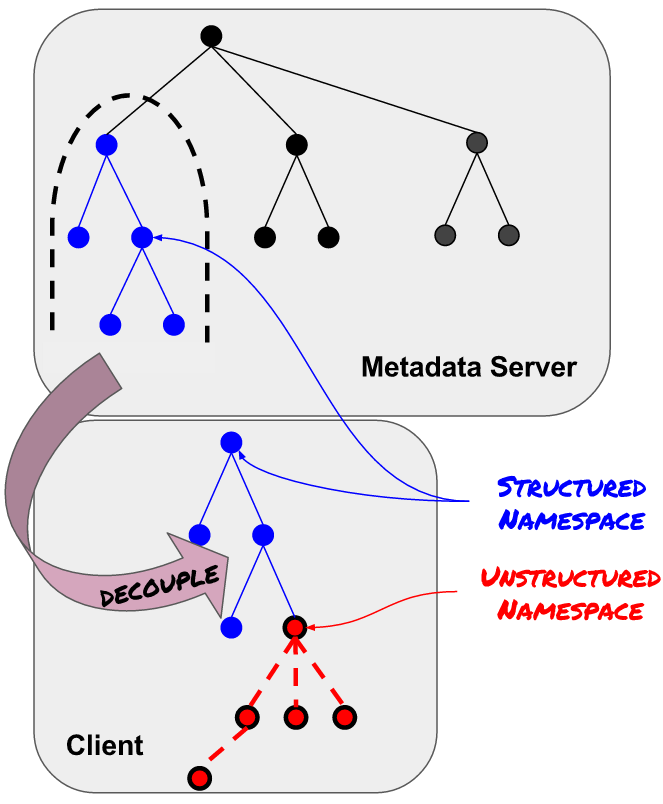
\includegraphics[width=0.9\linewidth]{figures/intro.png}
  \caption{In (1), clients decouple file system subtrees and interact with
their copies locally for high performance. In (2), clients and metadata servers
generate subtrees using ``namespace generators", thus reducing RPC load.
\label{fig:intro}}
\end{figure}

\begin{itemize}
  \setlength\itemsep{-0.5em}
\item we motivate our work (Section~\S\ref{sec:motivating-examples}) by
examining namespace descriptions and overheads for examples from different
domains (high performance computing, high energy physics, and large
simulations)
\item we define namespace schemas (Section~\S\ref{sec:namespace-schemas}) for
categorizing file system hierarchies and namespace generators
(Section~\S\ref{sec:namespace-generators}) to compact metadata, thus reducing
RPC amplification and facilitating lazy metadata generation when needed
\item a programmable storage approach that pushes user-defined functionality
into the storage system, facilitating application-specific storage stacks using
a `dirty-slate' approach
\end{itemize}
